\documentclass[11pt]{article}
\usepackage{graphicx}

\begin{document}
\title{Lesson 20: Fourier Analysis}
\author{Colt Bradley}
\date{}
\maketitle

\section{Part 1}

First we use Simpson's rule to compute the integral that defines the Fourier transform. 

\begin{equation}
A(f) = \int_{-\infty}^{\infty} a(t) e^{-2 \pi i f t}dt
\end{equation}

After computing this integral, we plot both the real and imaginary parts. To get both parts, we actually take the well known identity 
\begin{equation}
e^{i \theta} = \cos \theta - i\sin \theta
\end{equation}
We can then preform two integrals, one with the cosine replacing the exponential and corresponding to the real part and the other with the sine replacing the exponential. The graphs obtained for both $a(t) = \cos (6 \pi t) e^{-t^2}$ and $a(t) = \sin (6 \pi t) e^{-t^2}$. They peak where expected, and we can see the different structures present when we plot both the imaginary and real parts. 
\begin{figure}[ht]
\centering
\begin{tabular}{cc}
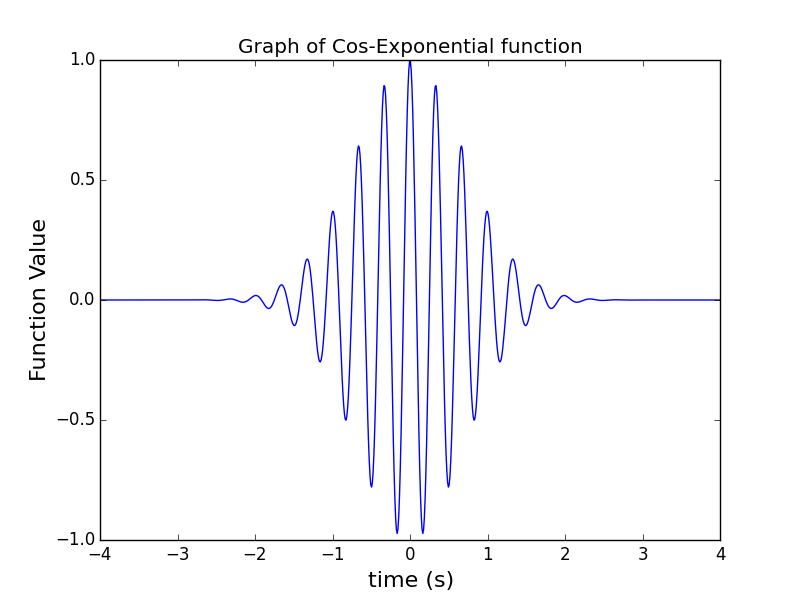
\includegraphics[scale=.4]{cos_wavepacket.png} \\
\multicolumn{2}{c}{(a) $a(t)$ vs time} \\[6pt]

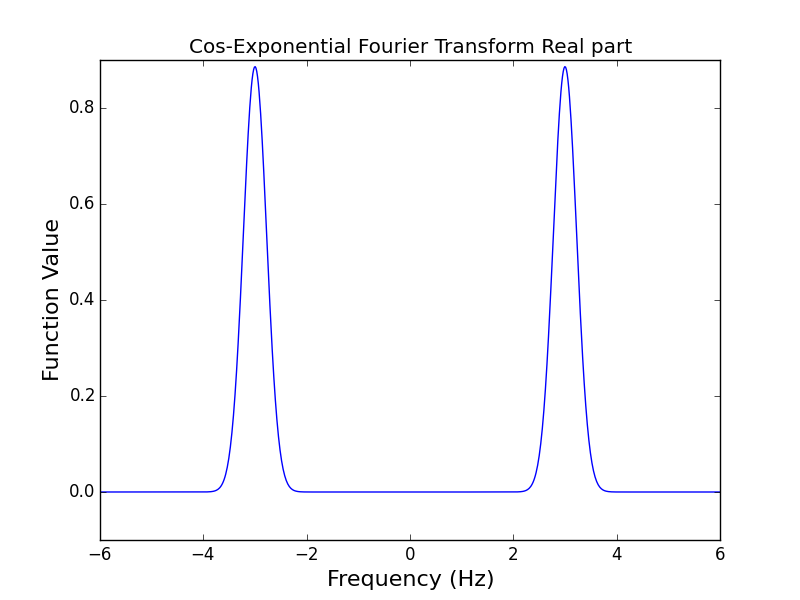
\includegraphics[scale=.4]{cos_fourReal.png}\\
\multicolumn{2}{c}{(b) Real part of $A(f)$ vs frequency} \\[6pt]

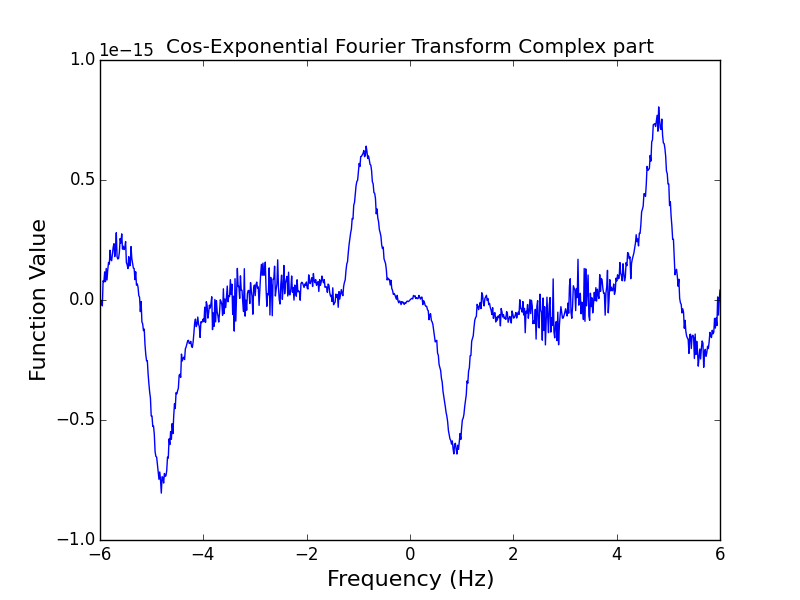
\includegraphics[scale=.4]{cos_fourComp.png}\\
\multicolumn{2}{c}{(c) Complex part of $A(f)$ vs frequency} \\[6pt]
\end{tabular}
\caption{Various plots for $\cos (6\pi t) e^{-t^2} $}
\end{figure}

\begin{figure}[ht]
\centering
\begin{tabular}{cc}
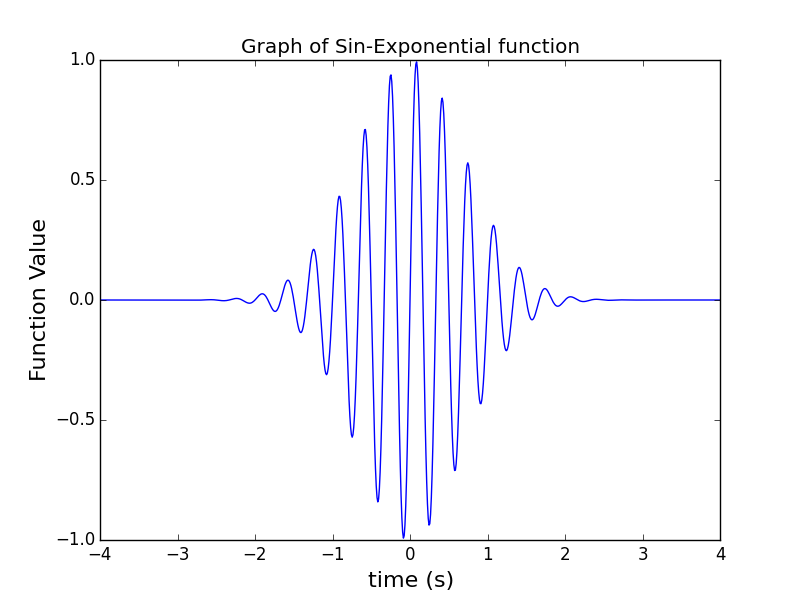
\includegraphics[scale=.4]{sin_wavepacket.png} \\
\multicolumn{2}{c}{(a) $a(t)$ vs time} \\[6pt]

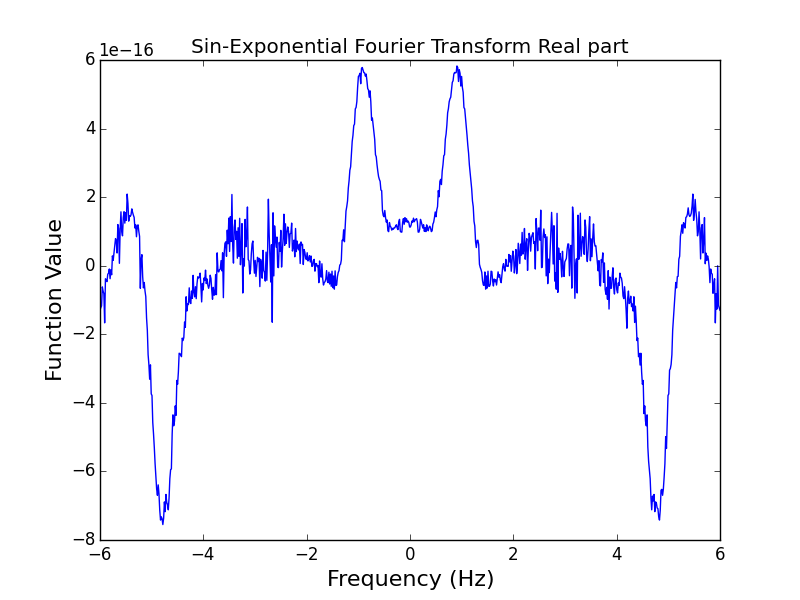
\includegraphics[scale=.4]{sin_fourReal.png}\\
\multicolumn{2}{c}{(b) Real part of $A(f)$ vs frequency} \\[6pt]

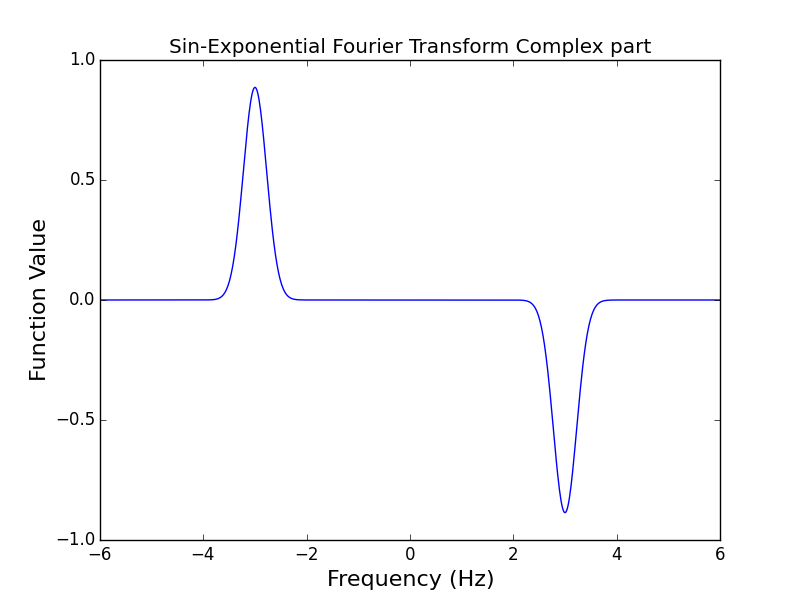
\includegraphics[scale=.4]{sin_fourComp.png}\\
\multicolumn{2}{c}{(c) Complex part of $A(f)$ vs frequency} \\[6pt]
\end{tabular}
\caption{Various plots for $\sin (6\pi t) e^{-t^2} $}
\end{figure}


\section{Part 2}

The answer to this part is very similar to part 1, but with different implementation. To compute this, we use python's fast Fourier transform function built into numpy. This time, we see two localized plectrums of frequencies in the real and imaginary parts. 

\begin{figure}[ht]
\centering
\begin{tabular}{cc}
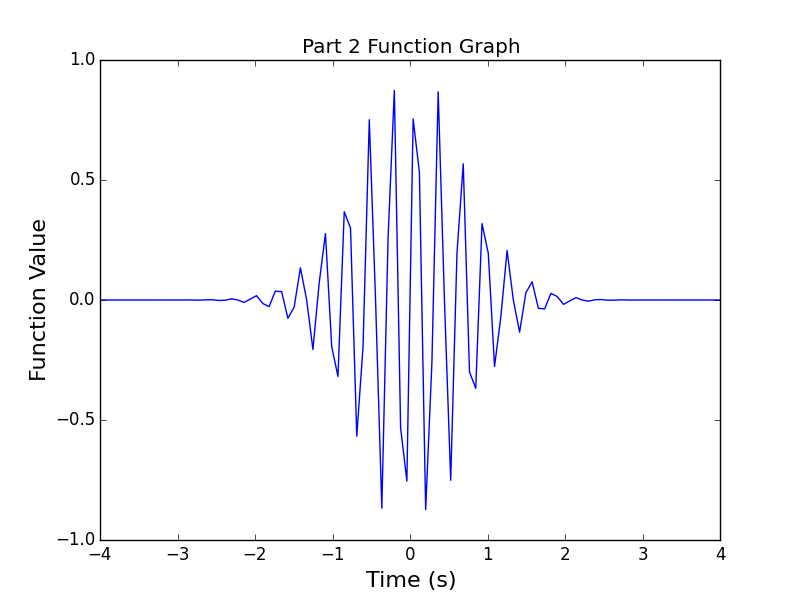
\includegraphics[scale=.4]{prt2_function.png} \\
\multicolumn{2}{c}{(a) $a(t)$ vs time} \\[6pt]

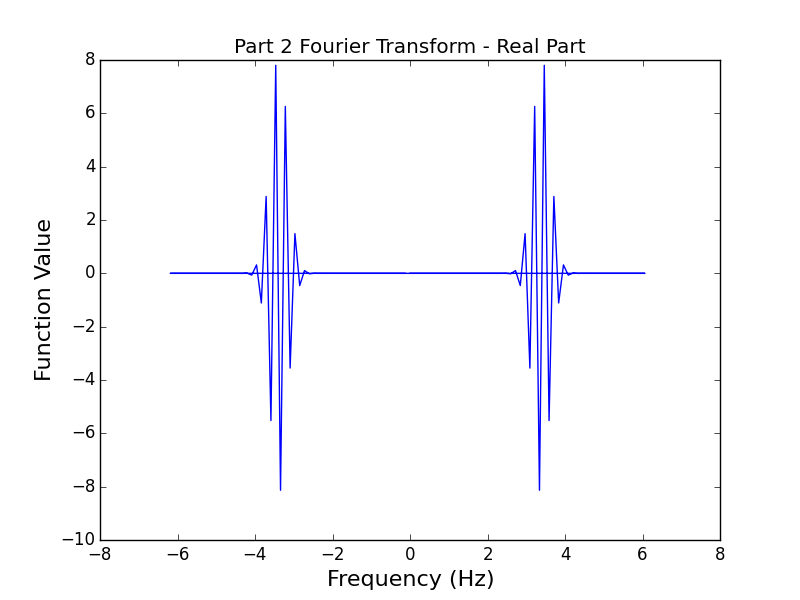
\includegraphics[scale=.4]{prt2_fourReal.png}\\
\multicolumn{2}{c}{(b) Real part of $A(f)$ vs frequency} \\[6pt]

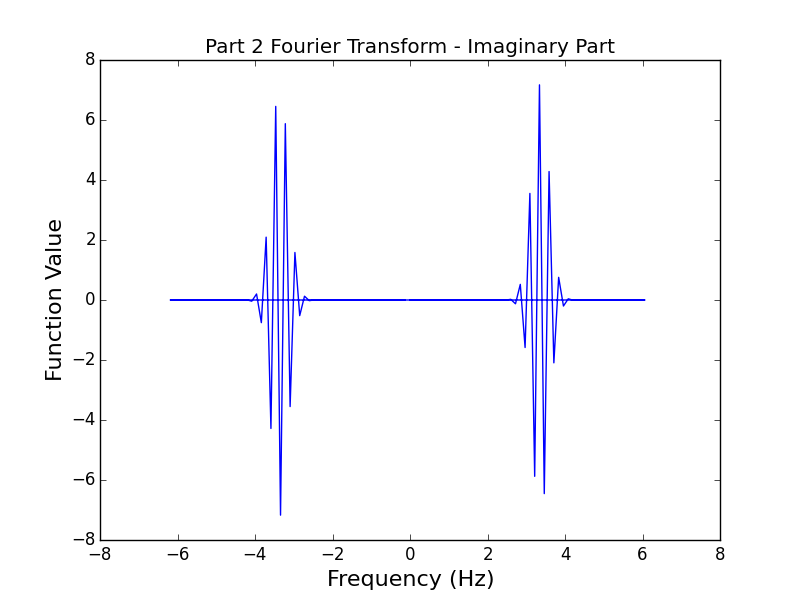
\includegraphics[scale=.4]{prt2_fourComp.png}\\
\multicolumn{2}{c}{(c) Complex part of $A(f)$ vs frequency} \\[6pt]
\end{tabular}
\caption{Various plots for $\cos (6\pi f_0 t) e^{-t^2} $}
\end{figure}

\section{Part 3}

Finally, we look at the imported data. We use the same fast Fourier transform method as described above, and we define a function that will calculate the power. 

Here, we see the frequency very sharply peaking at two points (around 5 and 1). These are the frequencies which comprise this signal. 

\begin{figure}[ht]
\centering
\begin{tabular}{cc}
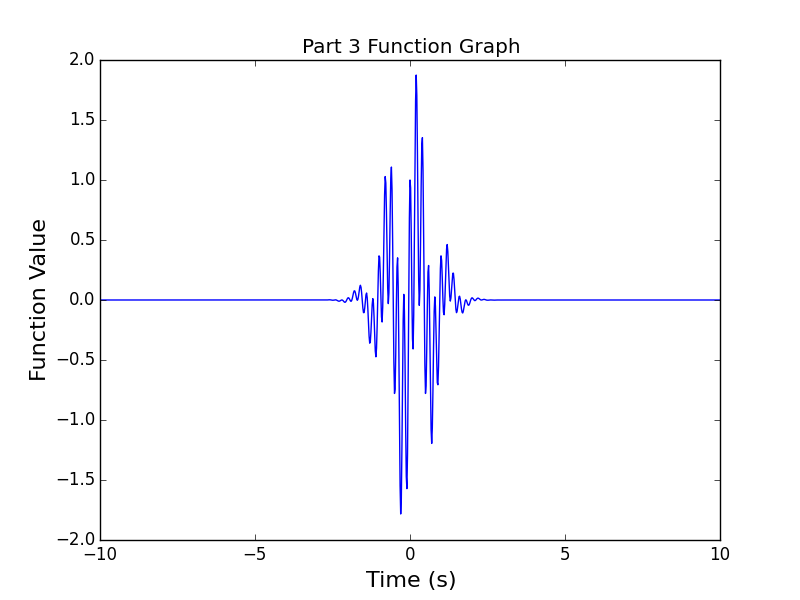
\includegraphics[scale=.4]{prt3_function.png} \\
\multicolumn{2}{c}{(a) data amplitudes vs time} \\[6pt]

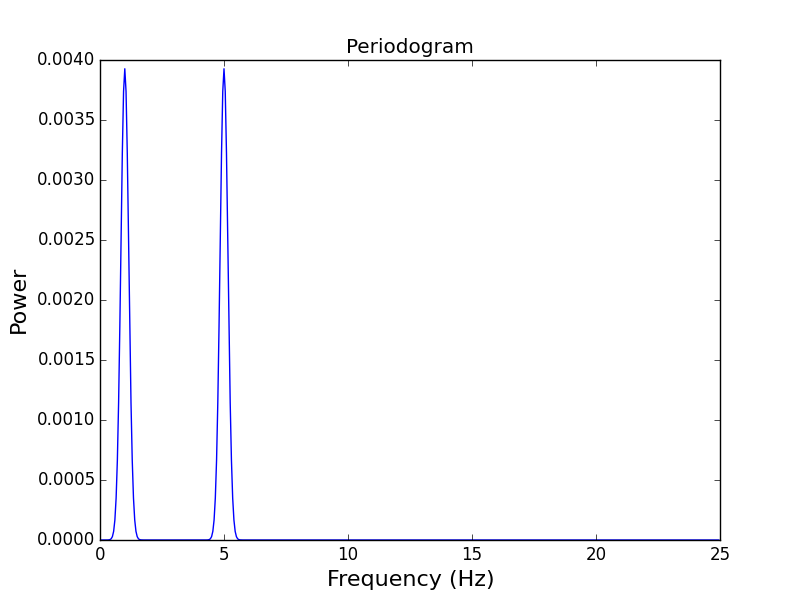
\includegraphics[scale=.4]{prt3_periodogram.png}\\
\multicolumn{2}{c}{(b) Periodogram} \\[6pt]

\end{tabular}
\caption{Various plots for imported data}
\end{figure}

\section{Codes}
\subsection{Part 1 Codes}
\begin{verbatim}
##Colt Bradley
#3.15.2016
#Lesson 20.1

import os
os.chdir("C:/Users/Colt/OneDrive/Documents/Professional/School/16spring/PY_251/20.FourierAnalysis")

#############################################################################
#functions and modules
#############################################################################
#import modules
import numpy as n
import pylab as p

#define essential functions
#first two are used in the first homeowrk exercise
def f(x):
    y = n.sin(6*n.pi*x)*n.exp(-x**2)
    return y
def g(x):
    y = n.cos(6*n.pi*x)*n.exp(-x**2)
    return y

    #These compute the real/complex parts of the fourier transform        
def fourReal(f,x,t):
    y = f(x)*n.cos(2*n.pi*x*t)
    return y
def fourComp(f,x,t):
    y = -f(x)*n.sin(2*n.pi*x*t)
    return y

#fucntion simpsonfour() is the simpson rule function specifically for fourier
def simpsonfour(f,g,t,a,b,N):
    h = float(b-a)/N
    i = 1
    n = 1
    
    I_1 = 0.
    while i < N:
        I_1 += f(g,a+i*h,t)
        i += 1
    
    I_2 = 0   
    while n < N+1:
        I_2 += f(g,a+n*h - h/2,t)
        n += 1
    return (h/6)*(f(g,a,t)+f(g,b,t)+2*I_1+4*I_2)


#############################################################################
#Homework 1
#############################################################################

#create a list of times
t1 = n.linspace(-4,4,num = 800)
func1 = []
func2 = []

for i in t1:
    func1.append(f(i))
    
for i in t1:
    func2.append(g(i))
    

#create a list to contain I, create a list for select numbers between the error
#function bounds
fReal = []
fComp = []
gReal = []
gComp = []
freq = n.linspace(-6,6,num = 800)

#compute the fourier transform for Real/complex part
for i in freq:
    k = simpsonfour(fourReal,f,i,-4,4,800)
    fReal.append(k)   
for i in freq:
    k = simpsonfour(fourComp,f,i,-4,4,800)
    fComp.append(k)
    
for i in freq:
    k = simpsonfour(fourReal,g,i,-4,4,800)
    gReal.append(k)
for i in freq:
    k = simpsonfour(fourComp,g,i,-4,4,800)
    gComp.append(k)
    
#Graph a(t) vs t for both functions
p.close()
p.plot(t1,func1,"b")
p.title("Graph of Sin-Exponential function")
p.xlabel("time (s)",fontsize = 16)
p.ylabel("Function Value",fontsize = 16)
p.savefig("sin_wavepacket.png")
p.show()

p.close()
p.plot(t1,func2,"b")
p.title("Graph of Cos-Exponential function")
p.xlabel("time (s)",fontsize = 16)
p.ylabel("Function Value",fontsize = 16)
p.savefig("cos_wavepacket.png")
p.show()

#Graph A(f) vs f real part
p.close()
p.plot(freq,fReal,"b")
p.title("Sin-Exponential Fourier Transform Real part")
p.xlabel("Frequency (Hz)",fontsize = 16)
p.ylabel("Function Value",fontsize = 16)
p.savefig("sin_fourReal.png")
p.show()

p.close()
p.plot(freq,gReal,"b")
p.title("Cos-Exponential Fourier Transform Real part")
p.xlabel("Frequency (Hz)",fontsize = 16)
p.ylabel("Function Value",fontsize = 16)
p.savefig("cos_fourReal.png")
p.show()

#Graph A(f) vs f Complex part
p.close()
p.plot(freq,fComp,"b")
p.title("Sin-Exponential Fourier Transform Complex part")
p.xlabel("Frequency (Hz)",fontsize = 16)
p.ylabel("Function Value",fontsize = 16)
p.savefig("sin_fourComp.png")
p.show()

p.close()
p.plot(freq,gComp,"b")
p.title("Cos-Exponential Fourier Transform Complex part")
p.xlabel("Frequency (Hz)",fontsize = 16)
p.ylabel("Function Value",fontsize = 16)
p.savefig("cos_fourComp.png")
p.show()

\end{verbatim}

\subsection{Part 2 Codes}

\begin{verbatim}
##Colt Bradley
#3.15.2016
#Lesson 20.2

import os
os.chdir("C:/Users/Colt/OneDrive/Documents/Professional/School/16spring/PY_251/20.FourierAnalysis")

#############################################################################
#functions and modules
#############################################################################
#import modules
import numpy as n
import pylab as p

#define essential functions
 #These compute the real/complex parts of the fourier transform        
def fourReal(f,x,t):
    y = f(x)*n.cos(2*n.pi*x*t)
    return y
def fourComp(f,x,t):
    y = -f(x)*n.sin(2*n.pi*x*t)
    return y
    
def a(x):
    y = n.sin(6*n.pi*3*x)*n.exp(-x**2)
    return y

#############################################################################
#Homework 2
#############################################################################
t = n.linspace(-4,4,100)
dt = t[1]-t[0]
func3 = []

for k in t:
    func3.append(a(k))

#computes the discrete transform
A = n.fft.fft(func3)
#changes time values to frequency
freq = n.fft.fftfreq(len(t),dt)

p.close()
p.plot(t,func3,"b")
p.title("Part 2 Function Graph")
p.xlabel("Time (s)",fontsize = 16)
p.ylabel("Function Value",fontsize = 16)
p.savefig("prt2_function.png")
p.show()

p.close()
p.plot(freq,n.real(A),"b")
p.title("Part 2 Fourier Transform - Real Part")
p.xlabel("Frequency (Hz)",fontsize = 16)
p.ylabel("Function Value",fontsize = 16)
p.savefig("prt2_fourReal.png")
p.show()

p.close()
p.plot(freq,n.imag(A),"b")
p.title("Part 2 Fourier Transform - Imaginary Part")
p.xlabel("Frequency (Hz)",fontsize = 16)
p.ylabel("Function Value",fontsize = 16)
p.savefig("prt2_fourComp.png")
p.show()
\end{verbatim}

\subsection{Part 3 Codes}
\begin{verbatim}
##Colt Bradley
#3.15.2016
#Lesson 20.3

import os
os.chdir("C:/Users/Colt/OneDrive/Documents/Professional/School/16spring/PY_251/20.FourierAnalysis")

#############################################################################
#functions and modules
#############################################################################
#import modules
import numpy as n
import pylab as p

#define essential functions
 #These compute the real/complex parts of the fourier transform        
def fourReal(f,x,t):
    y = f(x)*n.cos(2*n.pi*x*t)
    return y
def fourComp(f,x,t):
    y = -f(x)*n.sin(2*n.pi*x*t)
    return y

#############################################################################
#Homework 3
#############################################################################
time,amp = n.loadtxt("Lesson20_Data.txt",usecols = (0,1), unpack =True)
dt = time[1]-time[0]
power = []
N = len(time)

#computes the discrete transform
A = n.fft.fft(amp)
#changes time values to frequency
freq = n.fft.fftfreq(N,dt)

power.append((1.0/N**2)*((A[0]*n.conj(A[0]))))
for i in range(1,N/2-1):
    power.append((1.0/N**2)*((A[i]*n.conj(A[i]))+(A[N-i]*n.conj(A[N-i]))))

power.append((1.0/N**2)*((A[N/2]*n.conj(A[N/2]))))

#create plots
p.close()
p.plot(time,amp,"b")
p.title("Part 3 Function Graph")
p.xlabel("Time (s)",fontsize = 16)
p.ylabel("Function Value",fontsize = 16)
p.savefig("prt3_function.png")
p.show()

p.close()
p.plot(freq[:N/2+dt],power,"b")
p.title("Periodogram")
p.xlabel("Frequency (Hz)",fontsize = 16)
p.ylabel("Power",fontsize = 16)
p.savefig("prt3_periodogram.png")
p.show()

\end{verbatim}

\end{document}